% Appendicies =======================================
\ifpdf
    \graphicspath{{Appendix1/Figs/Raster/}{Appendix1/Figs/PDF/}{Appendix1/Figs/}}
\else
    \graphicspath{{Appendix1/Figs/Vector/}{Appendix1/Figs/}}
\fi

\chapter{Supplementary Data} 
\section*{Instrumentation}
\begin{figure}[h!]
    \begin{subfigure}{0.49\textwidth}
        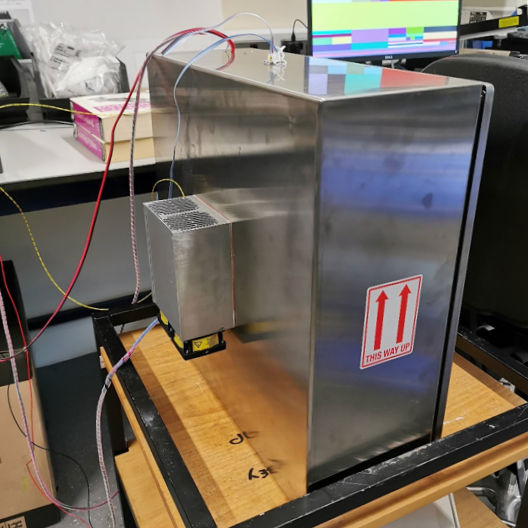
\includegraphics[width=\textwidth]{enclosure_back}
    \end{subfigure}
    \hspace*{\fill}
    \begin{subfigure}{0.49\textwidth}
        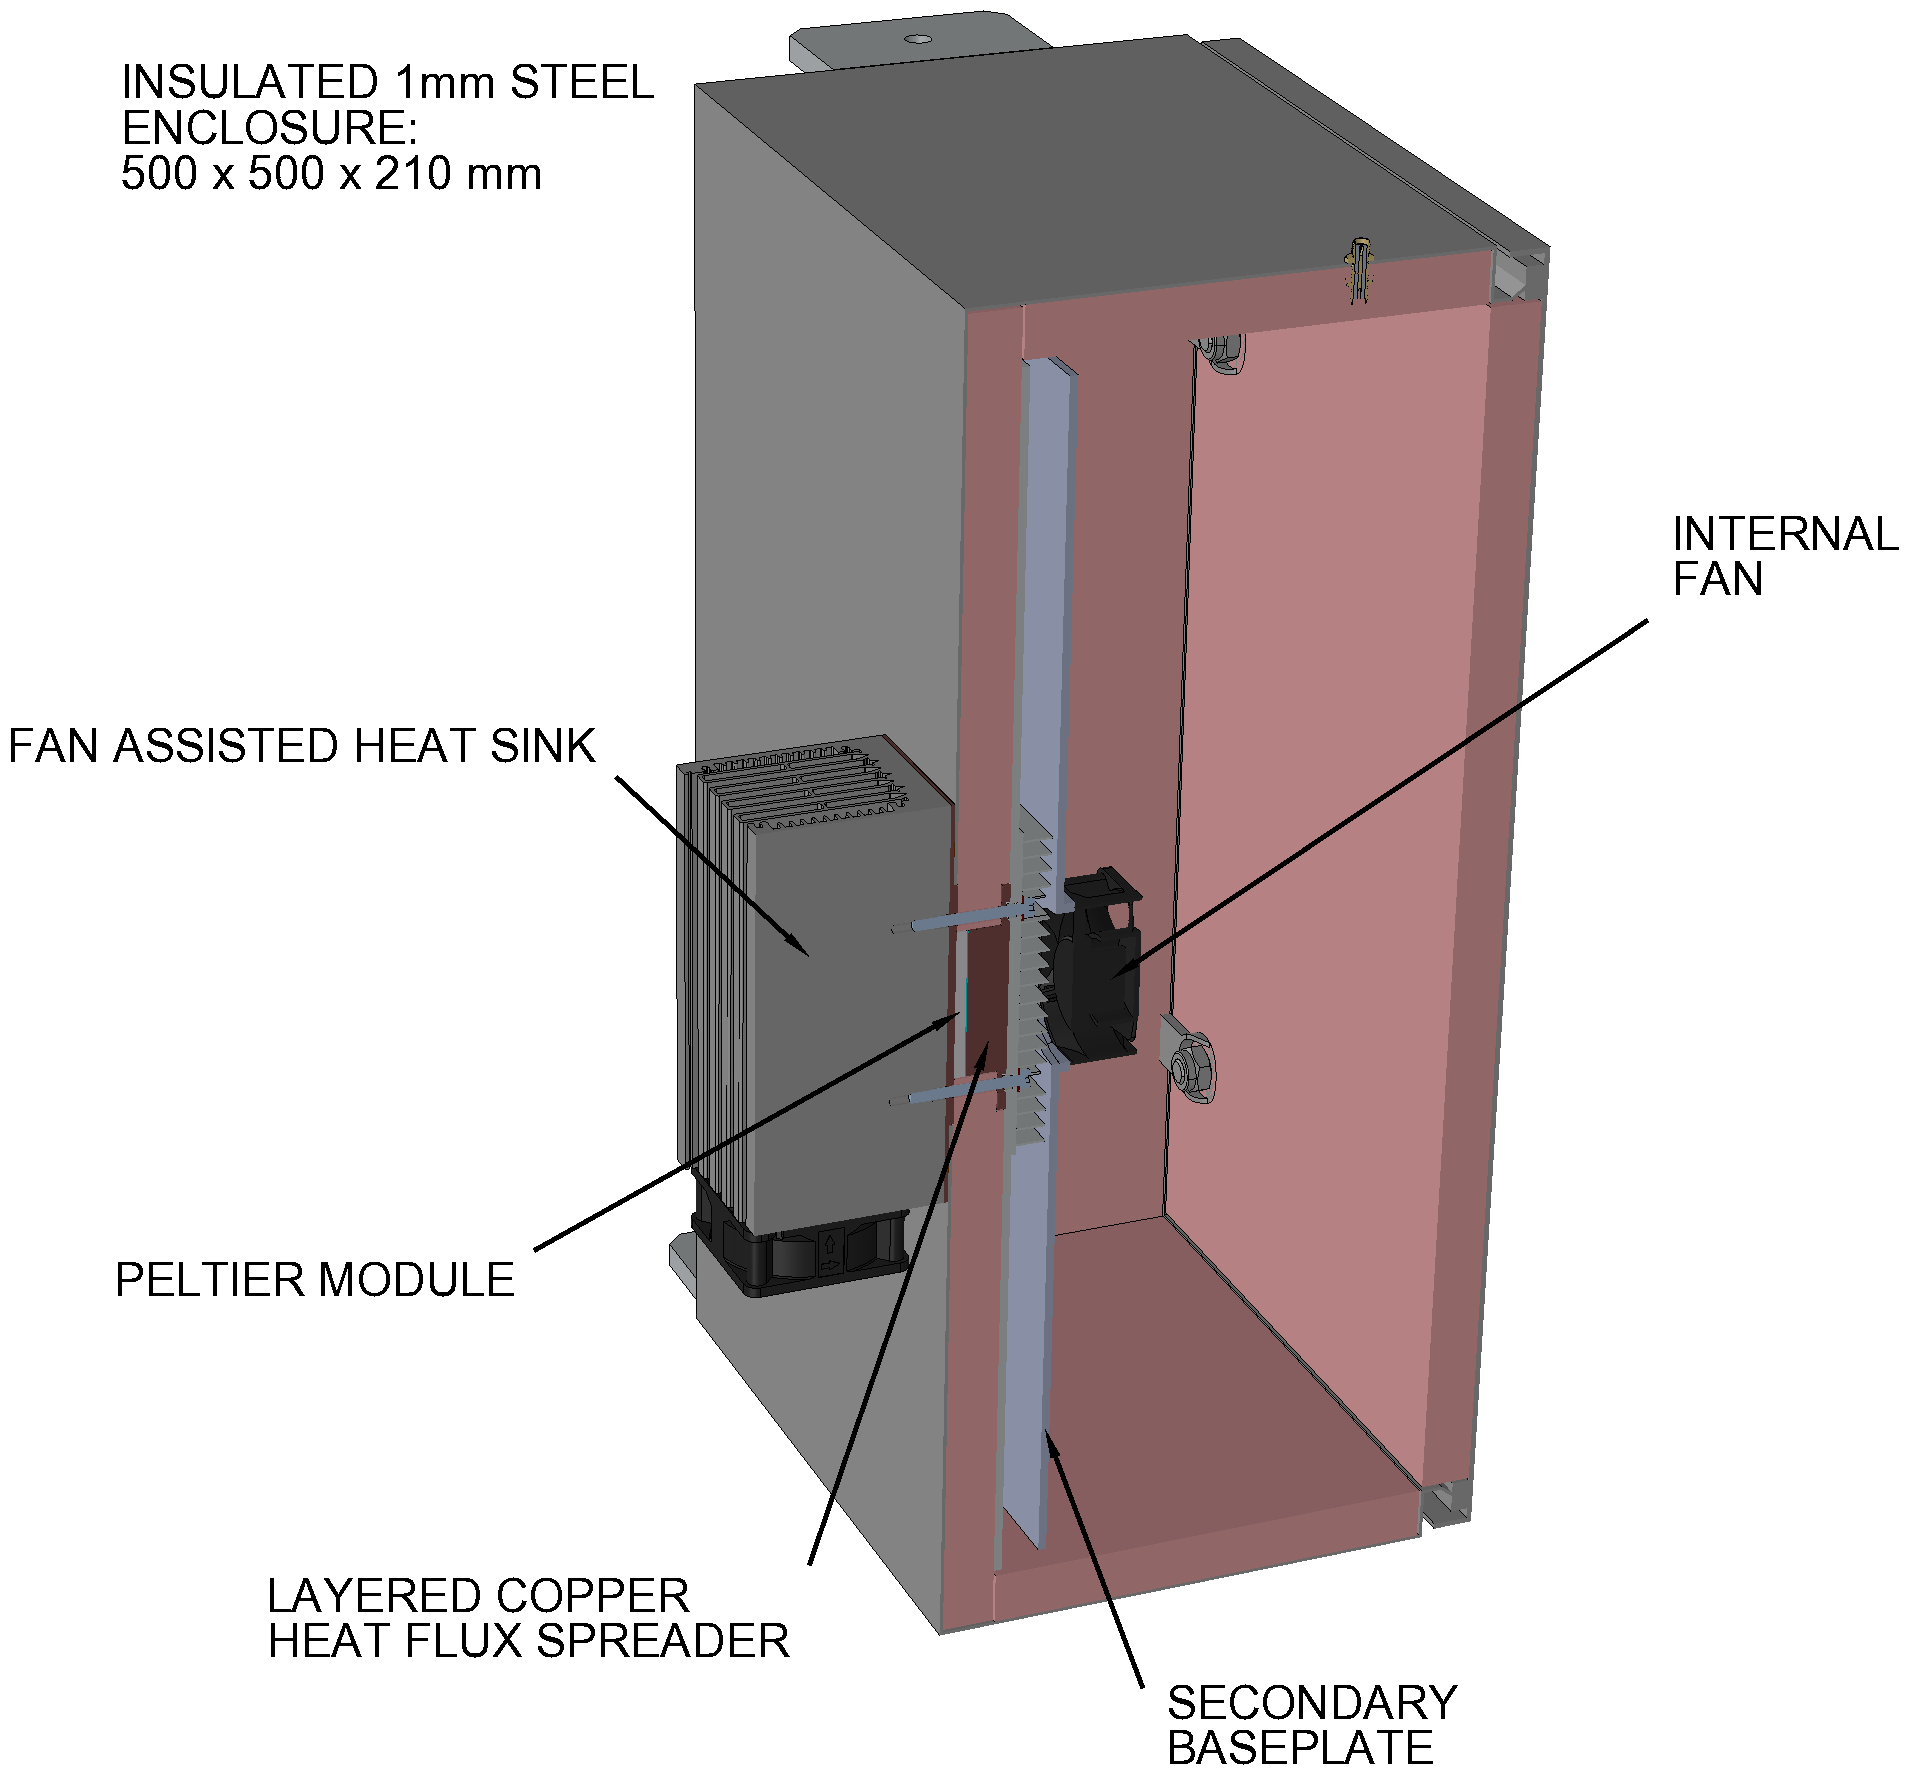
\includegraphics[width=\textwidth]{enclosure_cross_section}
    \end{subfigure}
    \caption{The completed front-end thermal enclosure is shown on the left. A 3D-rendered cross section in a similar orientation is shown on the right depicting the internal fan, baseplate, Peltier module and heat sink configuration. CAD rendering credit: Steven H. Carey.}
    \label{fig:enclose_supp}
\end{figure}


\begin{table}
    \begin{center}
    \begin{tabular}{ |c|c|c| }
    \hline
    Switch name & Model (Mini-Circuits) & Connection \\
    \hline
    MS1 & 12V MSP8TA-12-12D+ & Calibration sources \\
    MS2 & 24V MSP6TA-12D+& VNA path/calibration components \\
    MS3 & UNKNOWN & 2 metre cable terminations \\
    MS4 & UNKNOWN & 10 metre cable terminations \\
    MTS & 24V MTS-18XL-B+ & Spectrometer/VNA signal path \\
    \hline
    \end{tabular}
    \caption{Switch model number and connections from within the receiver front-end for reference. During the course of development, records of the model numbers for the MS3 and MS4 switches were lost.}
    \label{tab:switches}
    \end{center}
\end{table}

\begin{table}
    \begin{center}
    \begin{tabular}{ |c|c|c| }
        \hline
        {Switch} & {Position} & {Contents}\\
        \hline
        MS1 & 1 & Antenna \\
        MS1 & 2 & Heated $50 \Omega$ load \\
        MS1 & 3 & Reference noise source (diode) \\
        MS1 & 4 & Ambient $50 \Omega$ (cold) load \\
        MS1 & 5 & Ambient $25 \Omega$ load \\
        MS1 & 6 & Ambient $100 \Omega$ load \\
        MS1 & 7 & 2 metre calibration cable \\
        MS1 & 8 & 10 metre calibration cable \\
        \hline
        MS2 & 1 & MTS position 1 (towards calibration sources) \\
        MS2 & 2 & MTS position 3 (towards spectrometer path) \\
        MS2 & 3 & VNA calibration short \\
        MS2 & 4 & VNA calibration open \\
        MS2 & 5 & VNA calibration $50 \Omega$ load \\
        MS2 & 6 & VNA verification $50 \Omega$ test load \\
        \hline
        MS3 & 1 & $36 \Omega$ load \\
        MS3 & 2 & $27 \Omega$ load \\
        MS3 & 3 & $69 \Omega$ load \\
        MS3 & 4 & $91 \Omega$ load \\
        \hline
        MS4 & 1 & Open termination \\
        MS4 & 2 & Shorted termination \\
        MS4 & 3 & $10 \Omega$ load \\
        MS4 & 4 & $250 \Omega$ load \\
        \hline
        MTS & 1 & MS2 position 1 (calibration sources to VNA) \\
        MTS & 2 & MS1 (towards calibration sources) \\
        MTS & 3 & MS2 position 2 (LNA to VNA) \\
        MTS & 4 & Towards LNA (sources to spectrometer)\\
        \hline
    \end{tabular}
    \end{center}
    \caption{The content of each switch position for easy reference. This chart represents the receiver component positions at the time of the December 2022 deployment.}
    \label{tab:switch_content}
\end{table}

\begin{table}
    \centering
    \begin{tabular}{ |c|c|c| }
        \hline
        Power supply & Switchable & Component \\
        \hline
        3.3 V & No & Teensy 3.5 Development Board \\
        5 V & No & Fibre to USB converter \\
        6 V (A) & Yes & Low noise amplifier \\
        6 V (B) & Yes & Low noise amplifier \\
        12 V & Yes & VNA, RF switches \\
        24 V & Yes & Internal fan, RF switches \\
        28 V & Yes & Noise source diode \\
        \hline
    \end{tabular}
    \caption{Power supply considerations for the front-end receiver managed by the microcontroller unit. The ability to toggle the 5 V supply was disabled at the hardware-level in order to prevent accidental user activation which would result in a (catastrophic) completely non-responsive instrument.}
    \label{tab:power_supply}
\end{table}

\begin{figure}
    \centering
    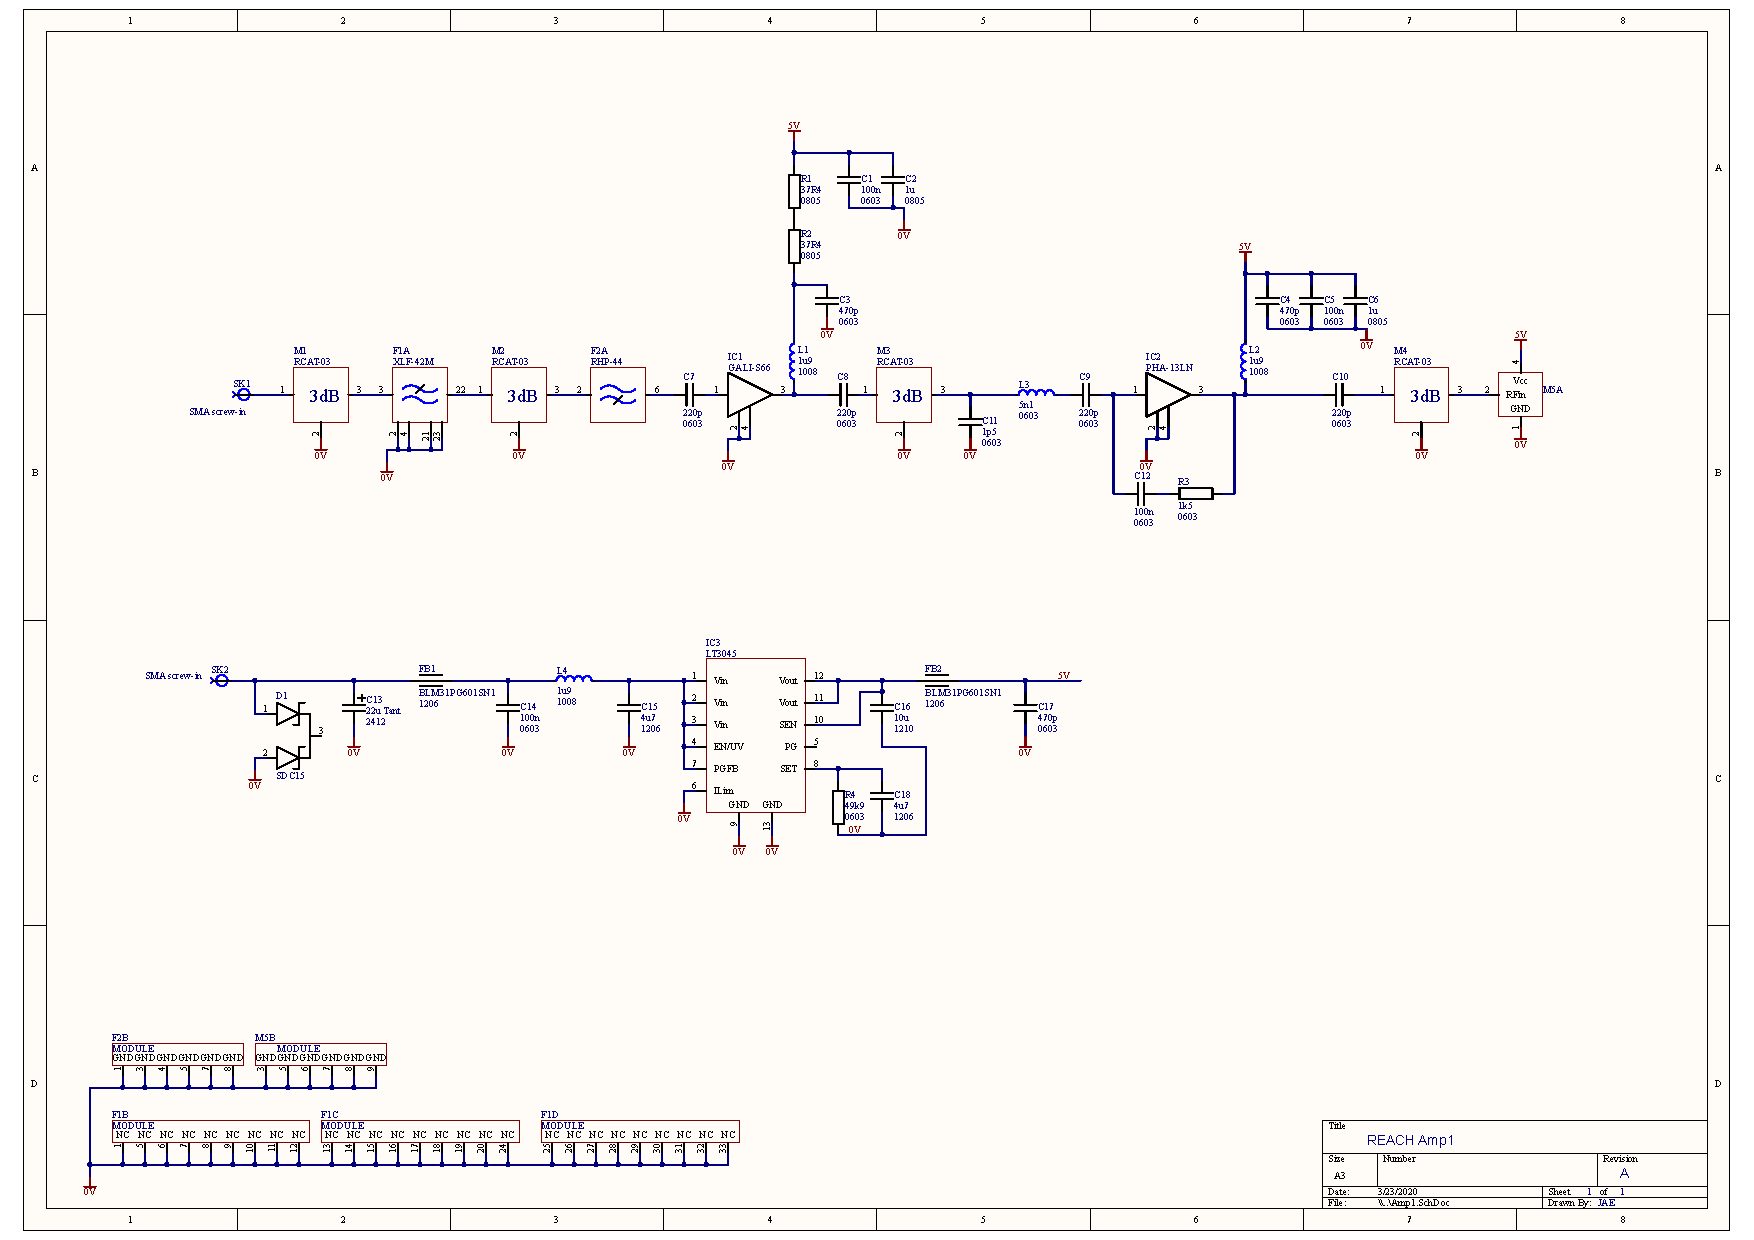
\includegraphics[angle=90,width=0.95\textwidth]{amp1_schematic}
    \caption{Full circuit diagram for amplifier \#1 in the REACH receiver front-end. Image credit: John A. Ely. Design credit: Nima Razavi-Ghods.}
    \label{fig:amp1_schematic}
\end{figure}

\begin{figure}
    \centering
    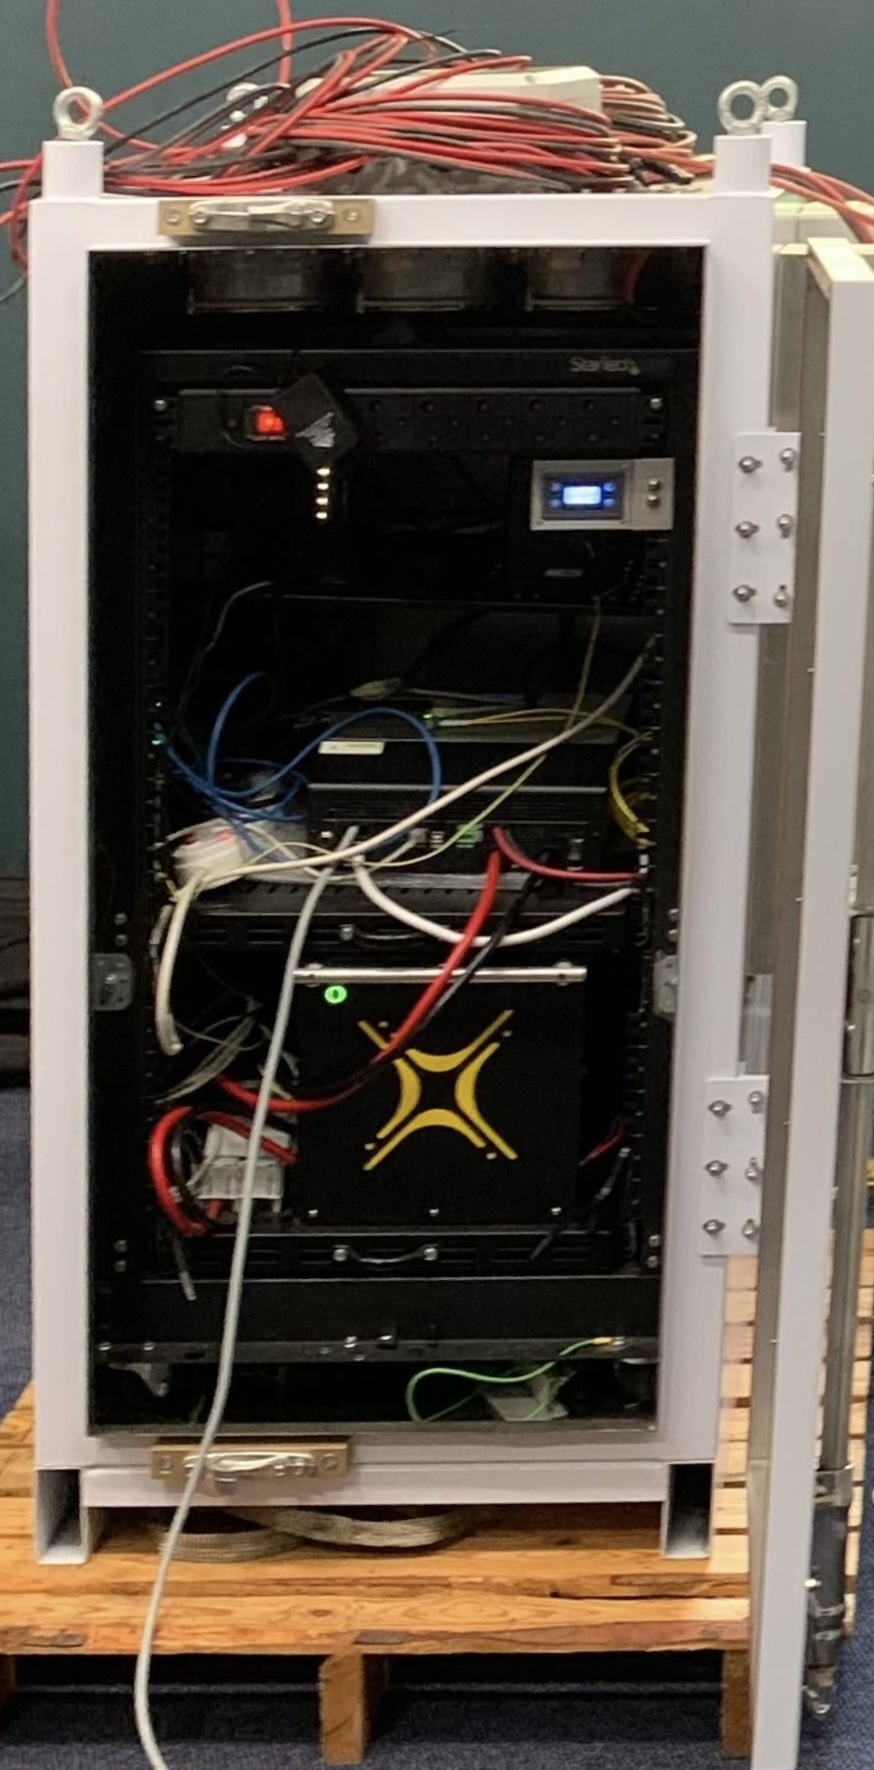
\includegraphics[scale=0.2]{power_chamber.jpeg}
    \caption{The smaller RF-EMC chamber accompanying the receiver back-end. This chamber houses various additional units for overnight power storage from the solar panels. The black module adorned with the yellow "X" symbol is the Solar MD SS202 Lithium Iron Phosphate battery.}
    \label{fig:power_chamber}
\end{figure}

\begin{figure}
    \centering
    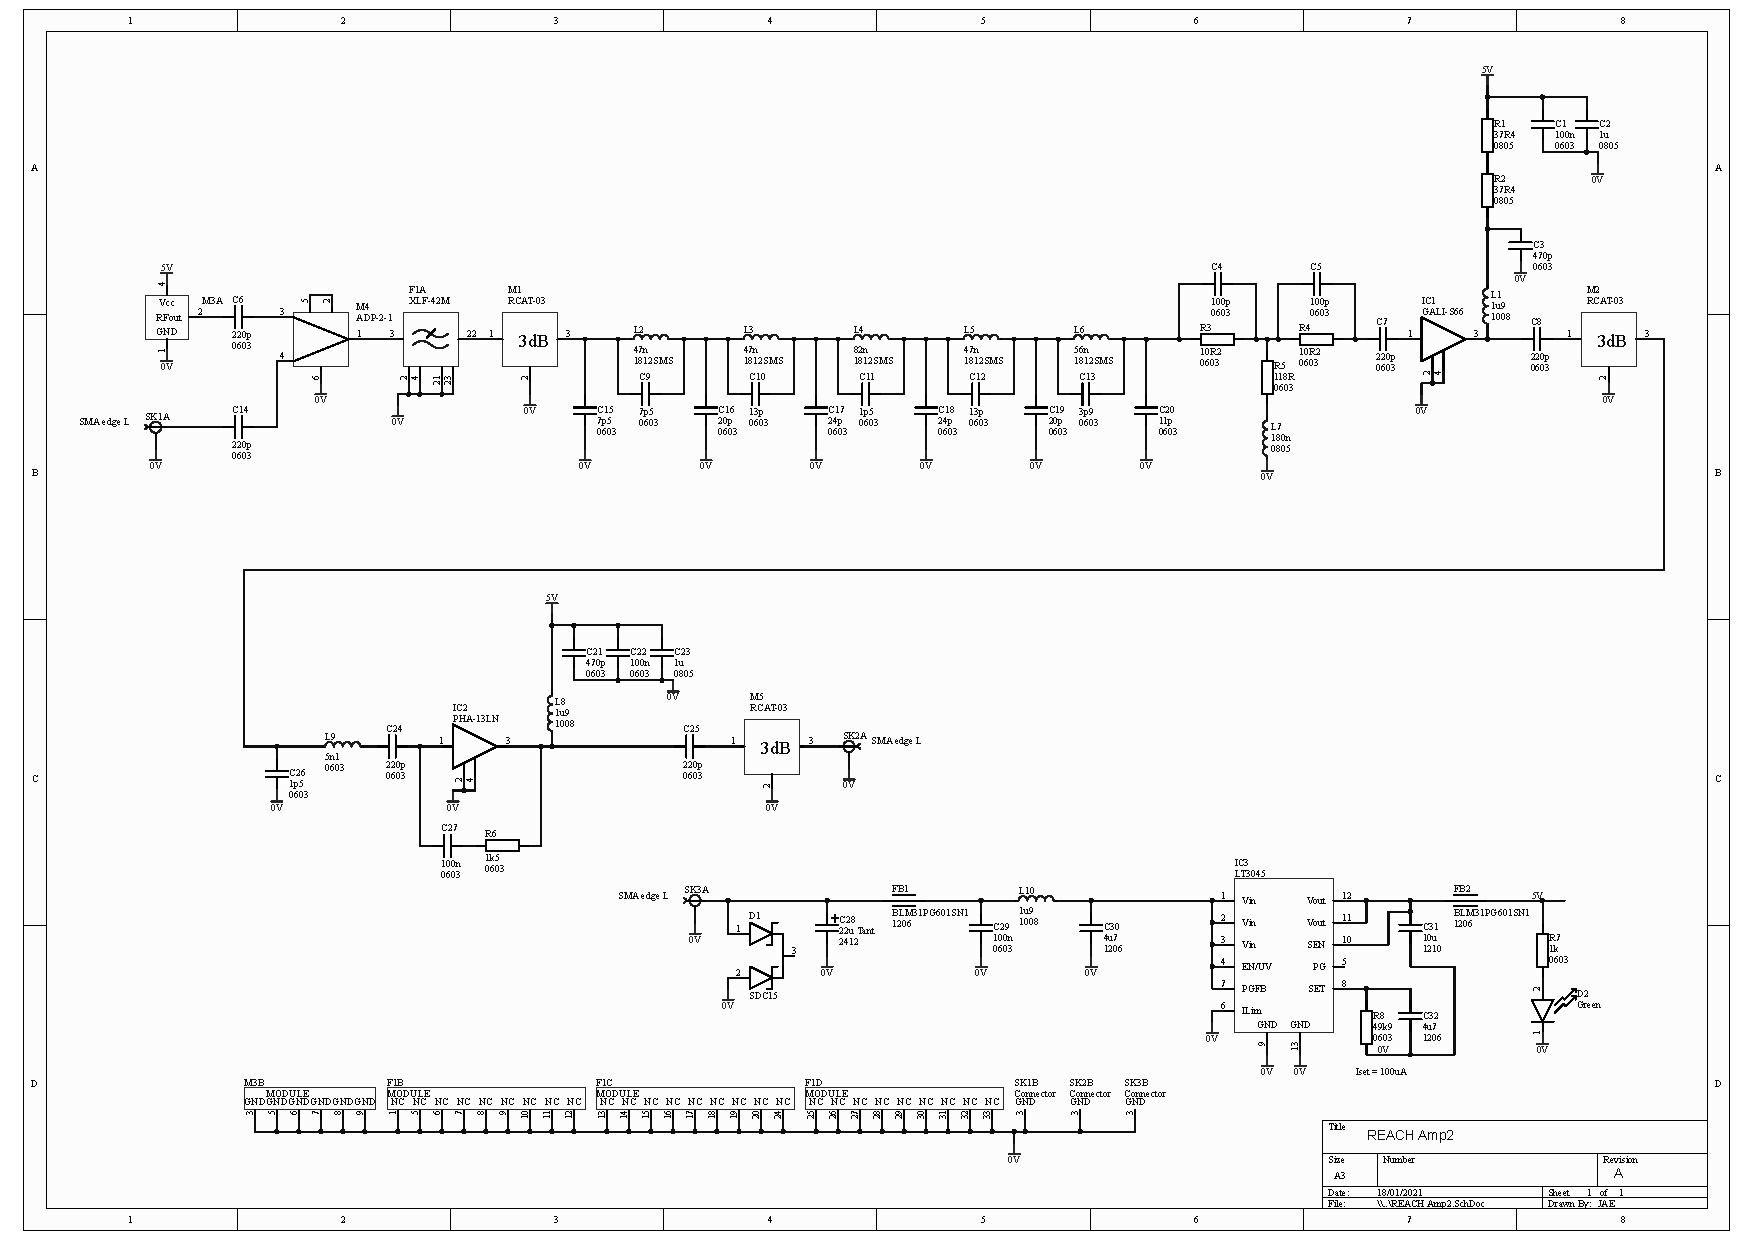
\includegraphics[angle=90,width=0.95\textwidth]{amp2_schematic}
    \caption{Full circuit diagram for amplifier \#2 in the REACH receiver back-end. Image credit: John A. Ely. Design credit: Nima Razavi-Ghods.}
    \label{fig:amp2_schematic}
\end{figure}

\begin{table}
    \begin{center}
    \begin{tabular}{ |c|c| }
    \hline
    Port Number & Device \\
    \hline
    7--24 V DC GND & Penn Elcom FT01-Q Cooling rack\\
    Port 0 & Lenovo ThinkCentre server \\
    Port 1 & ATEN CL6700 MW KVM module \\
    Port 2 & Netgear ProSafe M4100-D12G Ethernet switch \\
    Port 3 & Icron 2244 USB Ranger \\
    Port 4 & Unused \\
    Port 5 & Unused \\
    Port 6 & Readout system TEC controller USB connection \\
    Port 7 & Unused \\
    Port 8 & Unused \\
    Port 9 & Unused \\
    Port 10 & Unused \\
    \hline
    \end{tabular}
    \caption{Receiver back-end StarTech USB hub connections.}
    \label{tab:usb_hub}
    \end{center}
\end{table}

\begin{table}
    \begin{center}
    \begin{tabular}{ |c|c| }
    \hline
    Port Number & Device \\
    \hline
    Port 1 & Unused \\
    Port 2 & Readout system Ethernet output \\
    Port 3 & Unused \\
    Port 4 & Unused \\
    Port 5 & Unused \\
    Port 6 & Unused \\
    Port 7 & Lenovo ThinkCentre Ethernet input \\
    Port 8 & Unused \\
    Port 9 & Unused \\
    Port 10 & Unused \\
    Port 11 & Unused \\
    Port 12 & Tripp Lite PDUMH15HVNET power distribution unit \\
    \hline
    \end{tabular}
    \caption{Receiver back-end Netgear ProSafe M4100-D12G Ethernet switch connections.}
    \label{tab:eth_switch}
    \end{center}
\end{table}

\begin{table}
    \begin{center}
    \begin{tabular}{ |c|c| }
    \hline
    Port Number & Device \\
    \hline
    Port 1 & Penn Elcom FT01-Q cooling rack\\
    Port 2 & Netgear ProSafe M4100-D12G Ethernet switch (power connection) \\
    Port 3 & Lenovo ThinkCentre \\
    Port 4 & Icron 2244 USB Ranger \\
    Port 5 & Trimble Thunderbolt E GPS disciplined clock\\
    Port 6 & Readout enclosure power \\
    Port 7 & Second back-end power distribution unit \\
    Port 8 & ATEN CL6700 MW KVM module \\
    Ethernet port & Netgear ProSafe M4100-D12G Ethernet switch (Ethernet connection) \\
    \hline
    \end{tabular}
    \caption{Receiver back-end Tripp Lite PDUMH15HVNET power distribution unit connections.}
    \label{tab:backend_pdu}
    \end{center}
\end{table}

\begin{table}
    \centering
    \begin{tabular}{ |c|c|c| }
        \hline
        Frequency & Magnitude \\
        \hline 
        100 MHz & 71 dB \\
        200 MHz & 69 dB \\
        500 MHz & 61 dB \\
        1 GHz & 48 dB \\
        2 GHz & 32 dB \\
        3 GHz & 23.5 dB \\
        4 GHz & 15.5 dB \\
        \hline 
    \end{tabular}
    \caption{Voltage gain ($S_{21}$) for the custom built low noise amplifier used during initial calibration experiments detailed in \cref{sec:mphil_results}.}
    \label{tab:mphil_lna}
\end{table}

\begin{figure}
    \centering
    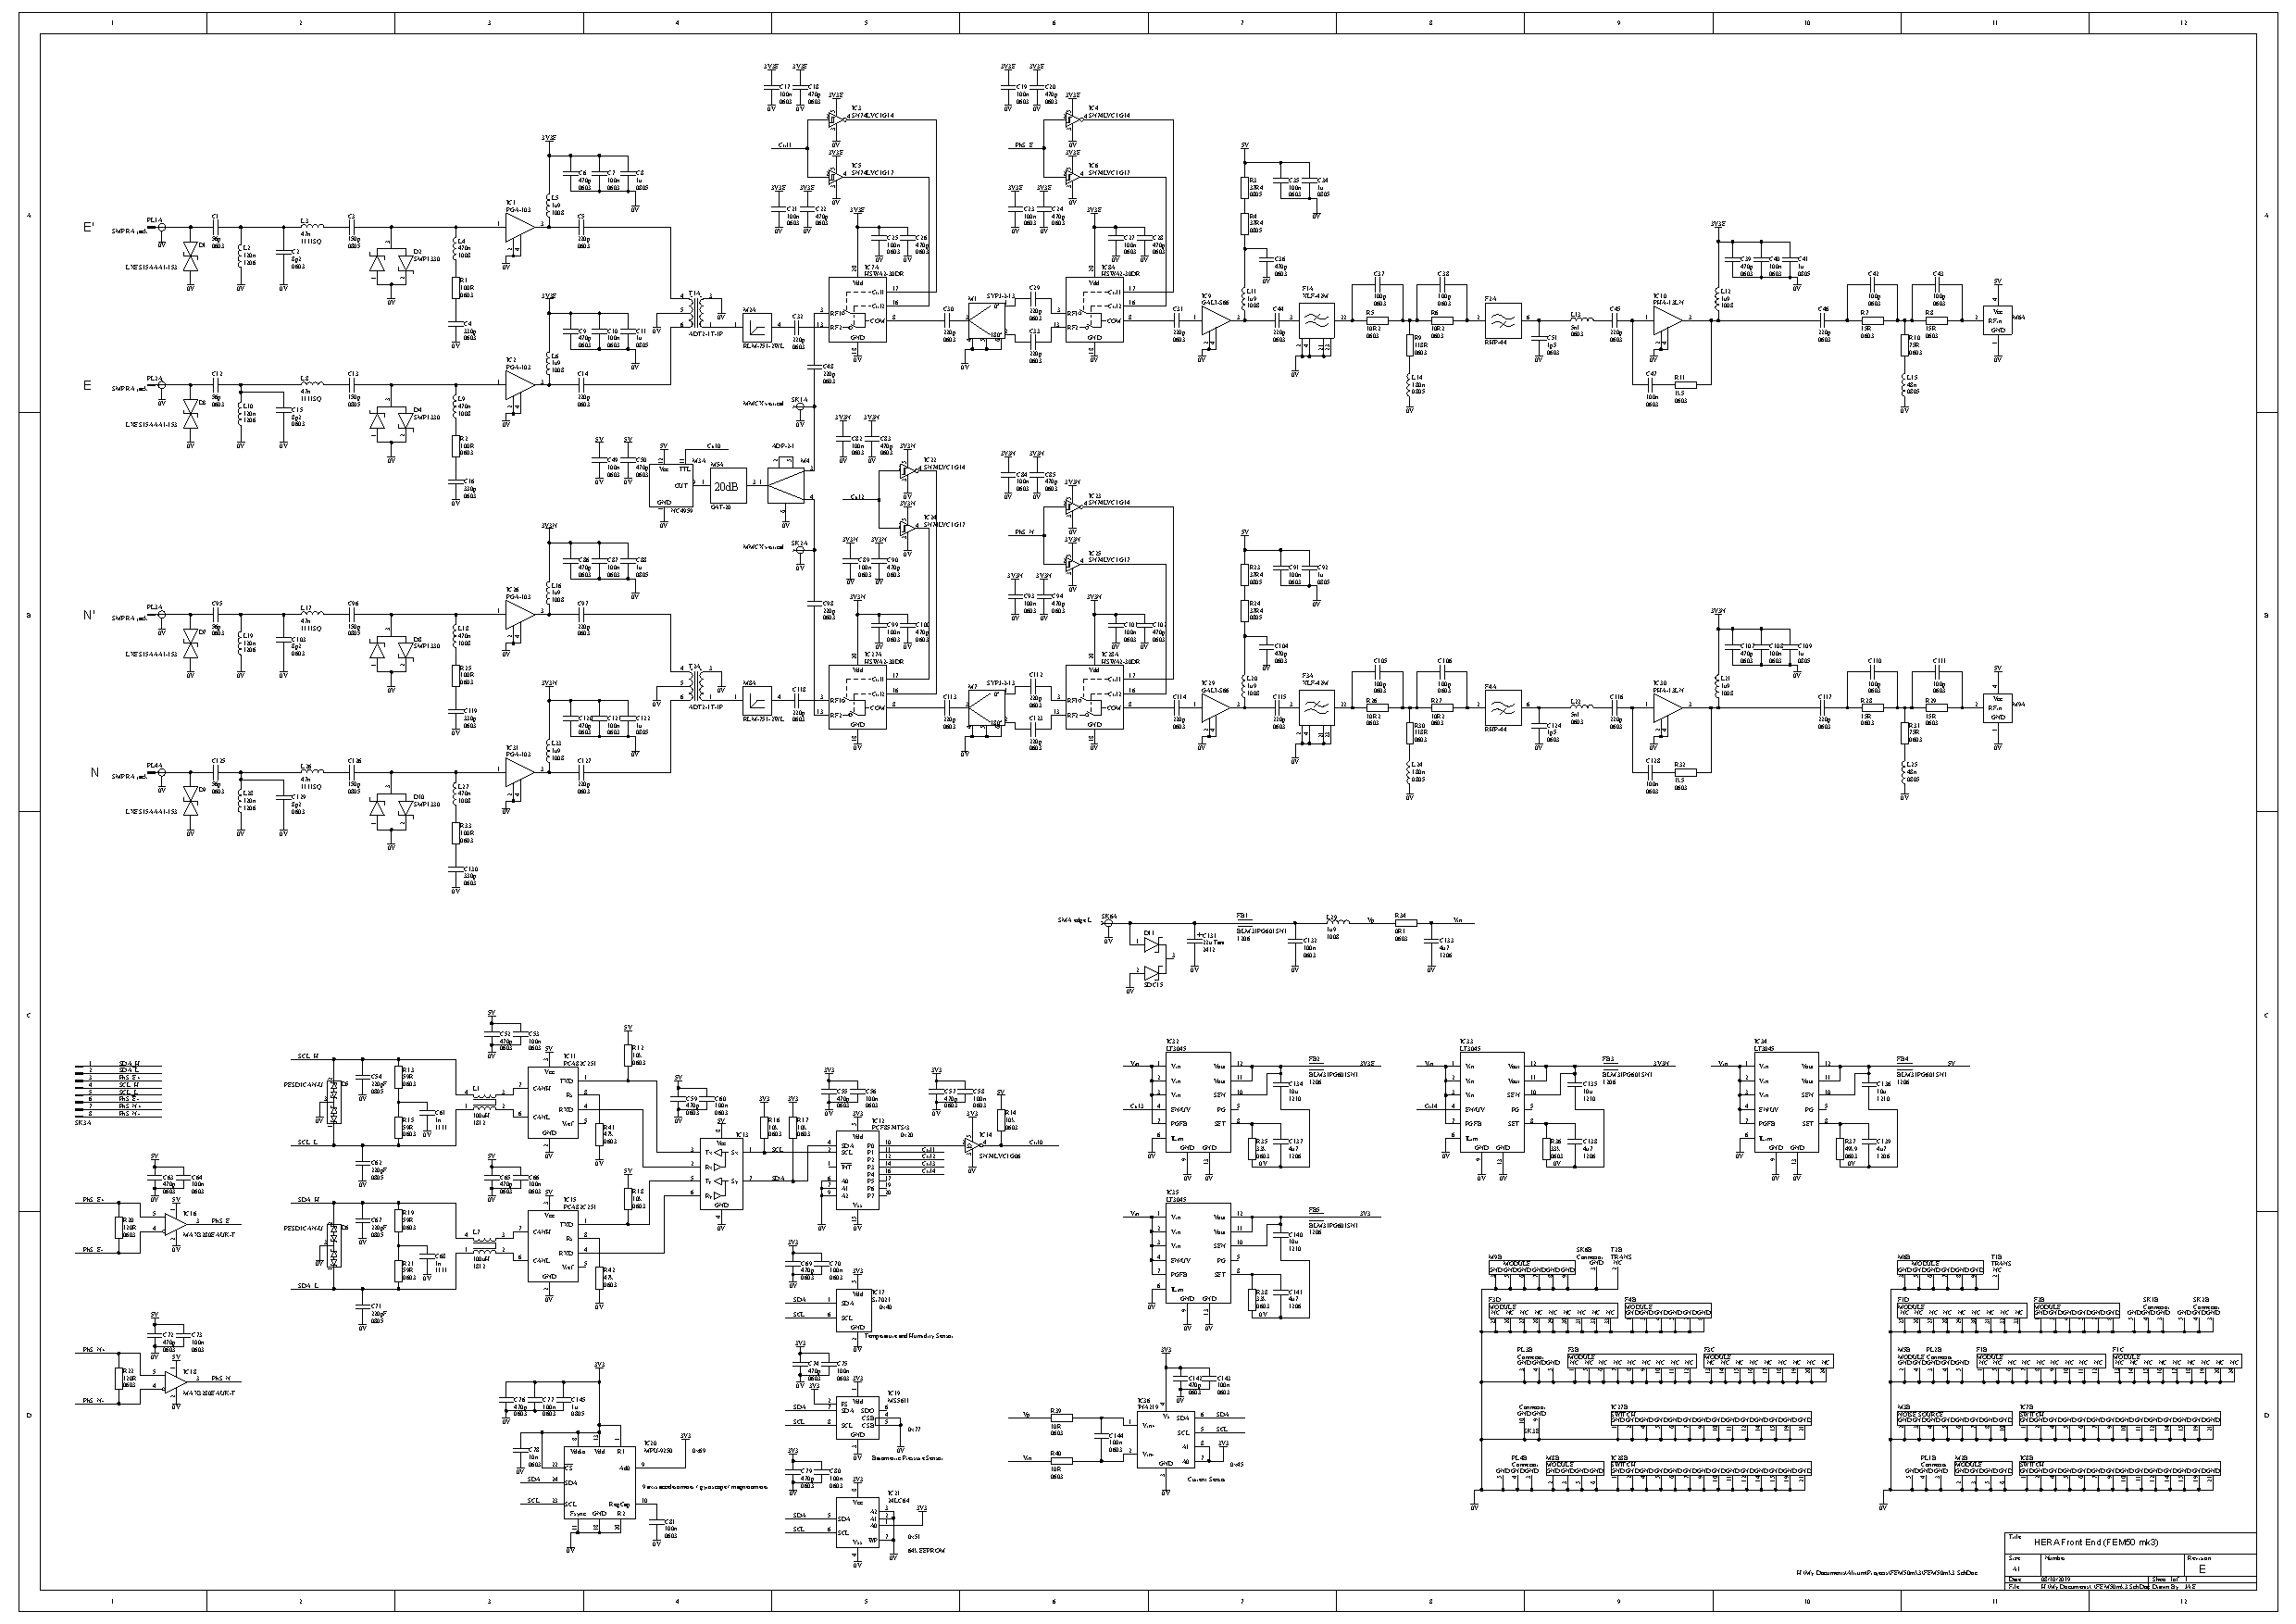
\includegraphics[angle=90,width=0.95\textwidth]{fem_schematic}
    \caption{Full circuit diagram for the HERA Front End Module mk III shown for reference. Image credit: John A. Ely. Design credit: Nima Razavi-Ghods.}
    \label{fig:fem_schematic}
\end{figure}

\begin{figure}
    \centering
    \begin{subfigure}{\textwidth}
        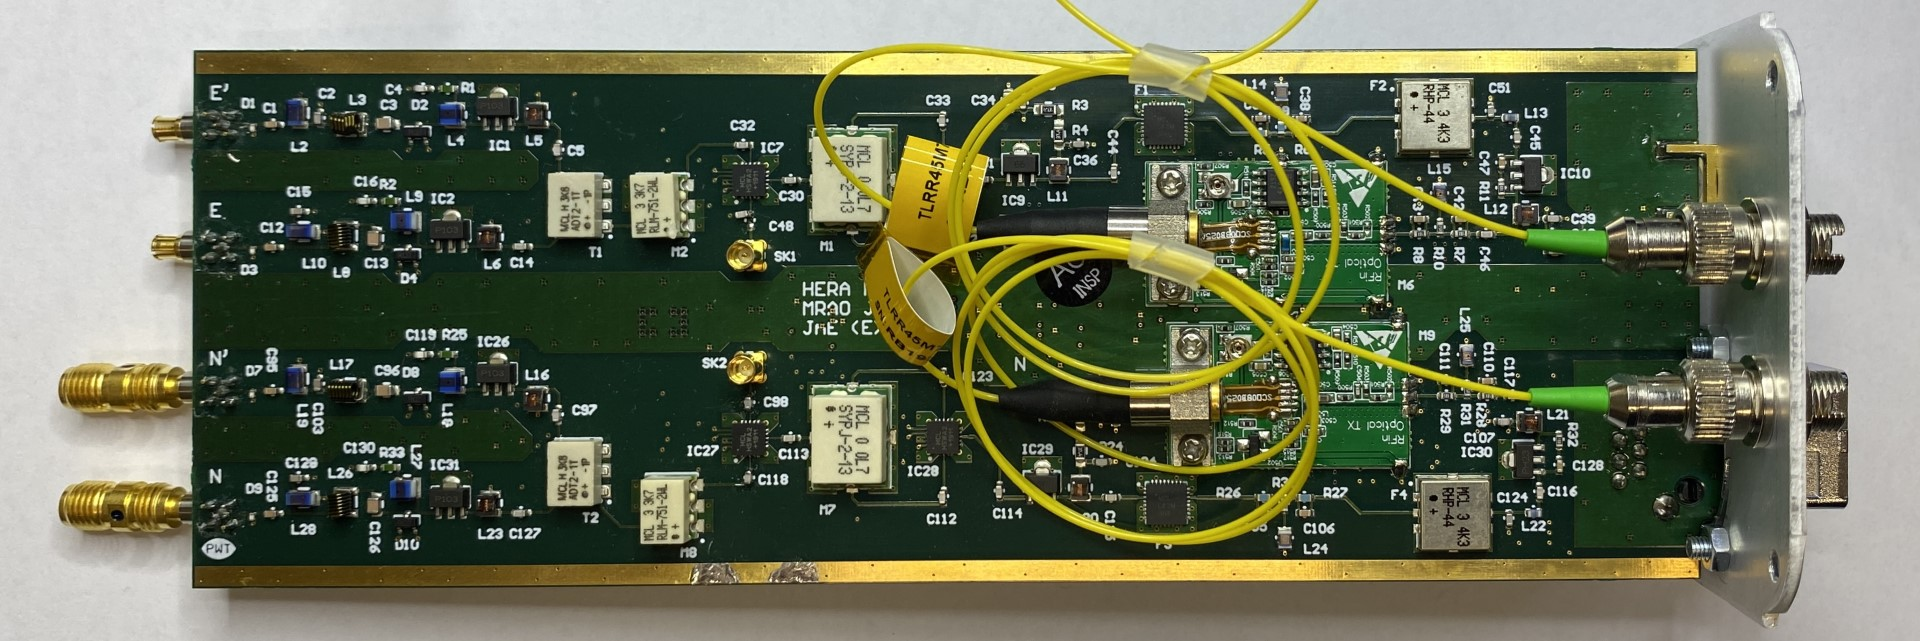
\includegraphics[width=\textwidth]{fem_top.jpg}
    \end{subfigure}
    \vspace{.5cm}
    \begin{subfigure}{\textwidth}
        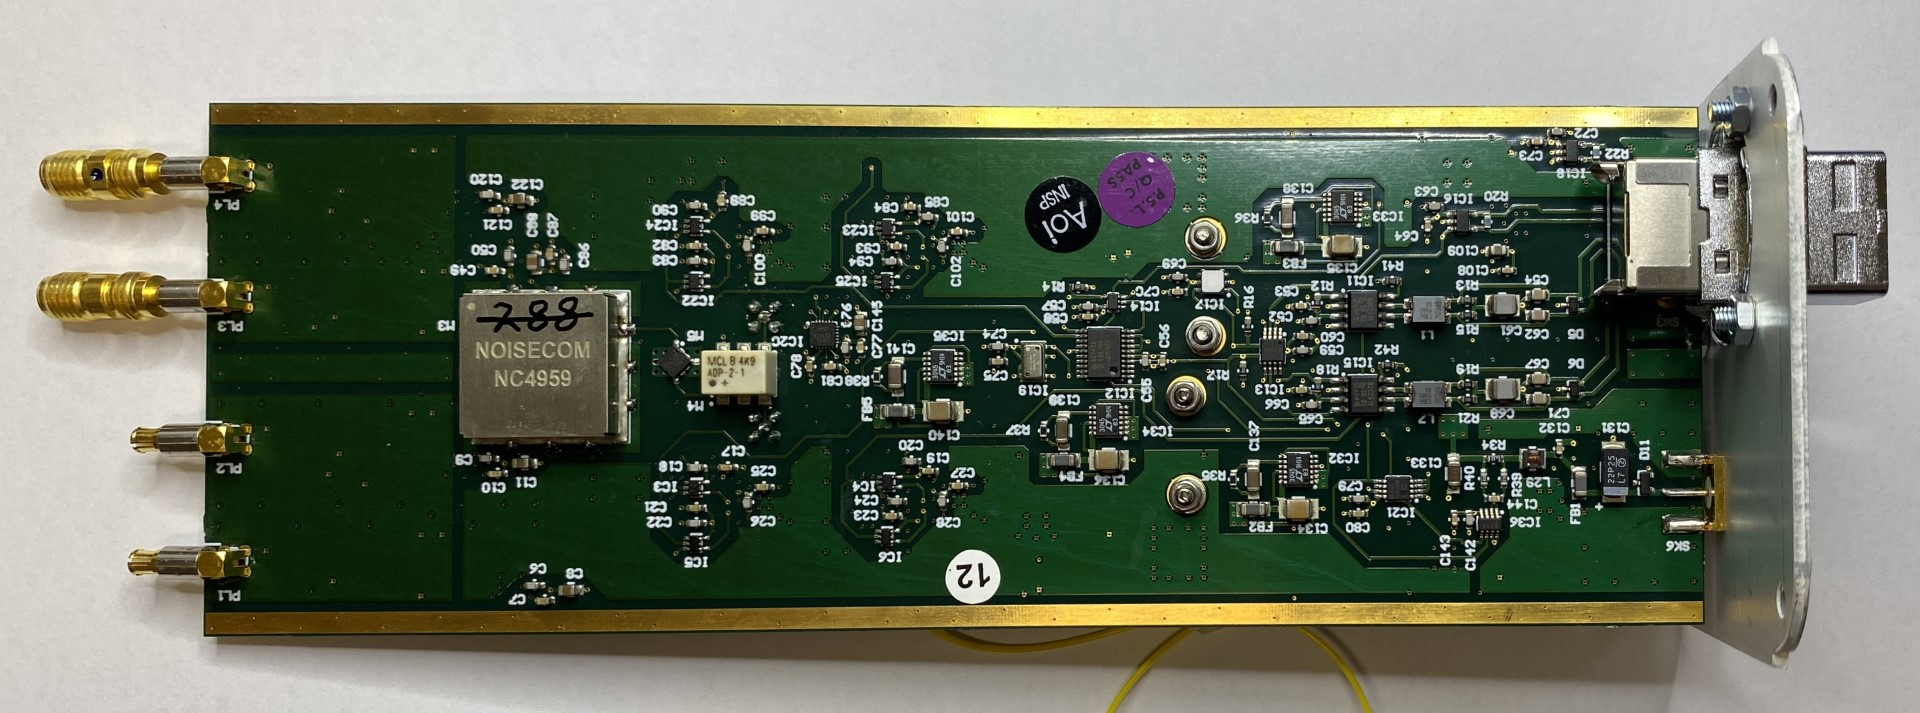
\includegraphics[width=\textwidth]{fem_bottom.jpg}
    \end{subfigure}
    \caption{The front and back of an unaltered HERA FEM board without its housing.}
    \label{fig:fem}
\end{figure}

\newpage\null\thispagestyle{empty}\newpage
